\documentclass[a4paper]{article}




%%%%%%%% CREATE DOCUMENT STRUCTURE %%%%%%%%
%% Language and font encodings
\usepackage[english]{babel}
\usepackage[utf8x]{inputenc}
\usepackage[T1]{fontenc}
%\usepackage{subfig}

%% Sets page size and margins
\usepackage[a4paper,top=3cm,bottom=2cm,left=2cm,right=2cm,marginparwidth=1.75cm]{geometry}

%% Useful packages

\usepackage{enumitem}
\usepackage{amsmath}
\usepackage{amssymb}
\usepackage{graphicx}
\usepackage[colorinlistoftodos]{todonotes}
\usepackage[colorlinks=true, allcolors=blue]{hyperref}
\usepackage{caption}
\usepackage{subcaption}
%\usepackage{sectsty}
%\usepackage{apacite}
\usepackage{float}
\usepackage{titling} 
\usepackage{blindtext}
\usepackage[square,sort,comma,numbers]{natbib}
\usepackage[colorinlistoftodos]{todonotes}
\usepackage{xcolor}
\usepackage{indentfirst}
\usepackage{amsmath}
\usepackage{mathtools}
\usepackage{tabularx}
\usepackage{array}
\usepackage{adjustbox}
%\usepackage{wrapfig}
\usepackage[linesnumbered,algoruled,boxed,lined]{algorithm2e}
\setlength\parskip{.5\baselineskip plus .1\baselineskip  minus .1\baselineskip}
\setlength{\parindent}{1em}
\definecolor{darkgreen}{rgb}{0.0, 0.4, 0.0}

\makeatletter
\def\BState{\State\hskip-\ALG@thistlm}
\makeatother

\DeclarePairedDelimiter\floor{\lfloor}{\rfloor}
\DeclarePairedDelimiter\ceil{\lceil}{\rceil}

\title{Kernel Based Learning Methods - Project}
\author{Alexander Parunov, Pau Rodríguez Esmerats }

%{\large \today}\\[2cm] % Date, change the \today to a set date if you want to be precise

%%%%%%%% DOCUMENT %%%%%%%%
\begin{document}


%
%----------------------------------------------------------------------------------------
%	HEADING SECTIONS
%----------------------------------------------------------------------------------------



\begin{minipage}{0.6\textwidth}
\begin{flushleft} \large
\textsc{\textbf{\Large Kernel Based Learning Methods }} - \textsc{\large Mid Term Project }\\[0.5cm] % Minor heading such as course title
\end{flushleft}
\end{minipage}
~
\begin{minipage}{0.4\textwidth}
\begin{flushright} \large
\includegraphics[scale=0.17]{img/fib2.png}\\[0.3cm]
\end{flushright}
\end{minipage}
 


\begin{minipage}{0.7\textwidth}
\begin{flushleft} 
\emph{Authors:}\\
Alexander Parunov, \\ Pau Rodríguez Esmerats
\end{flushleft}
\end{minipage}
~
\begin{minipage}{0.3\textwidth}
\begin{flushleft}
\emph{Date:}\\
\today
\end{flushleft}
\end{minipage}\\[0.5cm]


\section{Introduction}

In this project we are going to apply Kernel methods to a data analysis problem. Our work will be based on a research paper that builds a prediction model for the bit error rate(BER) in optical fiber communications in the event of a physical disturbance of a single fiber. We aim to build a new prediction model, that uses kernel methods to predict the value of the error rate.

The data set consists of the measurement of 3 variables of an optical fiber communication channel which are called State of Polarization (SOP), and the bit error rate measurement (BER). Those variables are gathered during periods of 4 seconds, during which a robotic arm that holds the optic fiber performs a physical action like rotation and or translation. The values are stored at a rate of 3600 values per second and there are a total of 360 experiments that last around 4 seconds each. The SOP variables are constrained to form a vector that lives in the unit sphere.

\section{Previous Work}

In the previous work, the researchers built a prediction model of the error rate based on 6 variables gathered in time windows of 10ms. Those variables consisted in :
\begin{itemize}
    \item the final value in the time window (at time t) of the 3 SOP variables
    \item the trends of each SOP within the time window [t-w,t]
\end{itemize}
The prediction goal was the BER value at $\delta$ ms after the last instance of the time windows. The values of the time window and the $\delta$ tested where between 10 and 300ms.
The variables and the BER where then discretized into p and q segments of equal length respectively. Then a Naive Bayes model is trained. Different hyper parameters of the model where tested. Accuracies obtained ranged from 3 to 12 percent.

\section{Predictive Model}

Different alternatives are proposed for this project:
\begin{itemize}
\item Classification model: a similar discretization could be performed on the value of the BER. For the variables, we could then use all the values of each SOP during a specific time window, with a specific granularity (for example: one value at each ms during a time window of 10 ms). In that case, an SVM model could be trained. One of the interesting points of this approach is to choose a powerful kernel that yields good results. We could also use a BER value from $t+\delta$ for a time window [t-w,t].
\item Regression model: we could avoid doing a discretization of the values and train a regression model using SVM for regression. We could also use a BER value from $t+\delta$ for a time window [t-w,t].
\item Time series prediction: we will base our work on a paper by  Müller, Vapnik et. al, which explains how to use support vector machines for time series prediction. 
\end{itemize}

\section{Preprocessing}

\subsection{Preprocessing steps}

The preprocessing will consist in the following steps:
\begin{enumerate}
\item Import data from multiple csv files into one data frame, selecting the columns related to the SOP and the error (BER)
\item Downsample the data from 1 value each 0.25ms to some reasonable value like 1 value each 1ms, 5ms or 10ms. We will consider also applying a moving average smoothing procedure to reduce noise, specially in the BER value.
\item Transform the dataset from 3 variables (SOP values) and one target (BER) to a dataset that contains w values from time t-w to time t for each SOP variables and for the BER, plus a value for the BER at time t+d.  We will select the values of w and d according to previous work,  applicability to the real case scenario where this model could be implemented and also suitability of the predictive models.
\end{enumerate}

\subsection{Downsampling and Moving average}



\begin{figure}[H]
\minipage{0.5\textwidth}%
  \centering
    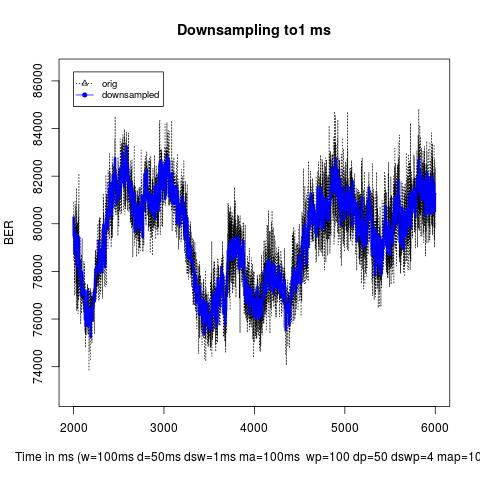
\includegraphics[width=0.9\linewidth]{img/downsampling_Time_in_ms_(w_100ms_d_50ms_dsw_1ms_ma_100ms__wp_100_dp_50_dswp_4_map_100).jpeg}
\endminipage\hfill
\minipage{0.5\textwidth}%
  \centering
    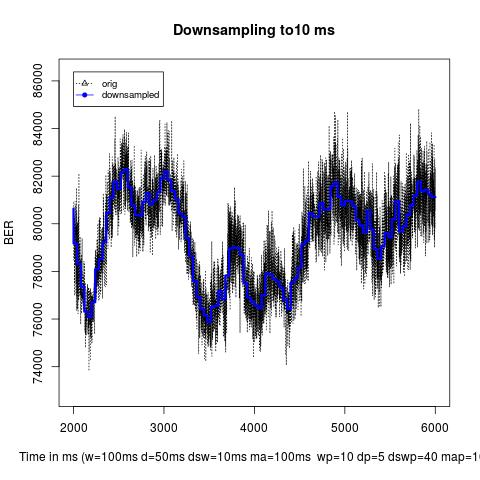
\includegraphics[width=0.9\linewidth]{img/downsampling_Time_in_ms_(w_100ms_d_50ms_dsw_10ms_ma_100ms__wp_10_dp_5_dswp_40_map_10).jpeg}
\endminipage\vfill
\minipage{0.5\textwidth}%
  \centering
    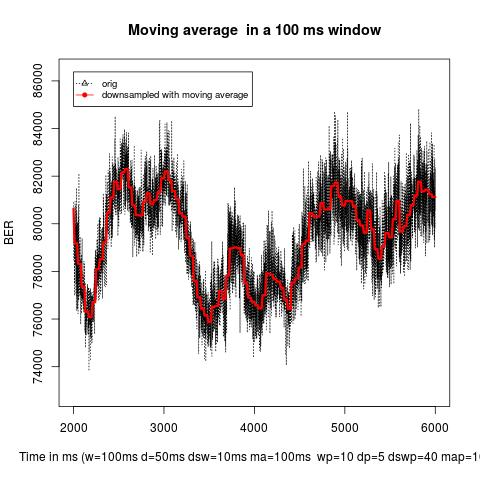
\includegraphics[width=0.9\linewidth]{img/ma_Time_in_ms_(w_100ms_d_50ms_dsw_10ms_ma_100ms__wp_10_dp_5_dswp_40_map_10).jpeg}
\endminipage\hfill
\minipage{0.5\textwidth}%
  \centering
    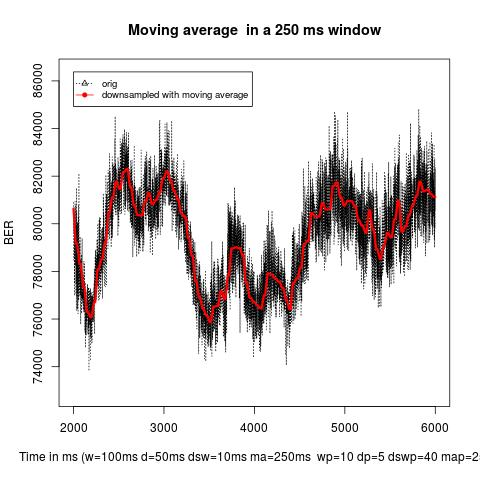
\includegraphics[width=0.9\linewidth]{img/ma_Time_in_ms_(w_100ms_d_50ms_dsw_10ms_ma_250ms__wp_10_dp_5_dswp_40_map_25).jpeg}
\endminipage

\caption{Ploting different downsampling rates and moving averages combined}
\end{figure}

We select the downsampling to 10ms rate as we consider it removes the a good quantity of noise in the target variable and at the same time maintains it's major trend accurately. We also observe that the variable signal will appear more smooth when applying a moving average of the previous values in the previous 250ms (depending on the downsampling rate selected, the number of data points to perform the average will vary).

\subsection{Transforming the dataset }
 We will transform the data set into a sequence of time series values for each SOP variable and the BER value in a time window from t-w to t. We will also add the future BER value in an instance t+d.
 The selected values that we will test the models on will be:
 \begin{itemize}
     \item w=50,100,200ms 
     \item d=50,100,200ms
 \end{itemize}

\end{document}





% %\vspace*{-15pt}
% \begin{figure}[H]
%     \centering
%     \includegraphics[width=0.8\linewidth]{img/Altmann.png}
%     \caption{Optimized parameters for the Altmann function for different initial values ranging from 0.01 to 50 in logarithmic increments}
%     \label{fig:altmann}
% \end{figure}
% %\vspace*{-15pt}



% \begin{figure}[H]
% \minipage{0.5\textwidth}%
%   \centering
%     \includegraphics[width=0.9\linewidth]{img/csn_task2_comm3200_walktrap.png}
%     \caption{Financial ratio related community}\label{com02}
% \endminipage\hfill
% \minipage{0.5\textwidth}%
%   \centering
%     \includegraphics[width=0.9\linewidth]{img/csn_task2_comm3202_walktrap.png}
%     \caption{Credit card related community}\label{com03}
% \endminipage
% \end{figure}\caption{Communities found with the Walktrap community detection algorithm}




